\documentclass[aspectratio=169,compress]{beamer}

\mode<presentation> {
	
	% The Beamer class comes with a number of default slide themes
	% which change the colors and layouts of slides. Below this is a list
	% of all the themes, uncomment each in turn to see what they look like.
	
	%\usetheme{default}
	%\usetheme{AnnArbor}
	%\usetheme{Antibes}
	%\usetheme{Bergen}
	%\usetheme{Berkeley}
%	\usetheme{Berlin}
	%\usetheme{Boadilla}
	%\usetheme{CambridgeUS}
	%\usetheme{Copenhagen}
%	\usetheme{Darmstadt} % Outline with circle progress on the top 
	%\usetheme{Dresden}
%	\usetheme{Frankfurt}
	%\usetheme{Goettingen}
%	\usetheme{Hannover} %option
	%\usetheme{Ilmenau}
	%\usetheme{JuanLesPins}
	%\usetheme{Luebeck}
	\usetheme{Madrid} %option
	%\usetheme{Malmoe}
	%\usetheme{Marburg}
	%\usetheme{Montpellier}
	%\usetheme{PaloAlto}
	%\usetheme{Pittsburgh}
	%\usetheme{Rochester}
%	\usetheme{Singapore} %option
	%\usetheme{Szeged}
	%\usetheme{Warsaw}
	
	% As well as themes, the Beamer class has a number of color themes
	% for any slide theme. Uncomment each of these in turn to see how it
	% changes the colors of your current slide theme.
	
%	\usecolortheme{albatross} %blue bk
%	\usecolortheme{beaver} %white, grey, red
%	\usecolortheme{beetle} %grey, white, blue
%	\usecolortheme{crane} %yellow, black
%	\usecolortheme{dolphin} %w,b,k
%	\usecolortheme{dove} %k,w,gray
%	\usecolortheme{fly} %gray bk
%	\usecolortheme{lily} % white bk, blue font
%	\usecolortheme{orchid} %default
%	\usecolortheme{rose}
%	\usecolortheme{seagull} %gray
%	\usecolortheme{seahorse} %lightblue
%	\usecolortheme{whale} %orchild-like
	\usecolortheme{wolverine} %orchild-like,yellow
	
	%\setbeamertemplate{footline} % To remove the footer line in all slides uncomment this line
	%\setbeamertemplate{footline}[page number] % To replace the footer line in all slides with a simple slide count uncomment this line
	
	\setbeamertemplate{navigation symbols}{} % To remove the navigation symbols from the bottom of all slides uncomment this line
    %	Progress on the top
	\useoutertheme[subsection=false]{miniframes}
	}

\graphicspath{{logo/}{figures/}{../../doc/sphinx/source/_figures/H2ONaCl}{../../doc/sphinx/source/_figures/IAPWS96_phi}{../../doc/sphinx/source/_figures/NaCl}} % figure path
\usepackage{graphicx}
\usepackage[center]{caption}

\usepackage{fontspec}
\setsansfont{Arial}

\usefonttheme[onlymath]{serif} % equation font

\usepackage{multicol} %	multiple columns

\usepackage{booktabs} % Allows the use of \toprule, \midrule and \bottomrule in tables
\usepackage{threeparttable}

\usepackage{mfirstuc} %	Captial first
\MFUnocap{are}
\MFUnocap{is}
\MFUnocap{of}

\usepackage{xcolor-material} %	Google theme color
\usepackage{calligra} % Thank you
\usepackage{natbib} % refernece
\renewcommand{\bibsection}{}%remove bib section from the top
	
\setbeamertemplate{navigation symbols}{} %remove navigation on the bottom

%\setbeamertemplate{footline} %remote author and title from the bottom
\usepackage{xcolor-material}
% Code highlight
\usepackage{minted}
% svg
\usepackage[inkscapearea=page]{svg}
%tikz plot
\usepackage{tikz}
\usetikzlibrary{arrows}
\usepackage[edges]{forest}
\usetikzlibrary{shapes, arrows, positioning}
\def\tikzarrow{\tikz[baseline=-0.6ex] \draw[arrows=-stealth,line width=1pt] (0ex,0ex) -- (3ex,0ex); }
\usepackage[many]{tcolorbox}
\usetikzlibrary{shadows}
\def\emcolor{blue}
\definecolor{darkgreen}{cmyk}{0.8,0,0.8,0.45}
\definecolor{lightgreen}{cmyk}{0.8,0,0.8,0.25}
\newtcolorbox{shadedbox}{
	drop shadow southeast=darkgreen,
	breakable,
	enhanced jigsaw,
	colback=white,
	colframe=lightgreen
}
% 1. set theme color
\setbeamercolor{block title}{bg=yellow!50,fg=black}
\definecolor{GEOMARlightblue}{RGB}{40,184,231}
\definecolor{GEOMARdarkblue}{RGB}{12,102,185}
\setbeamercolor*{palette primary}{bg=lightgray!50,fg=black}    
\setbeamercolor*{palette secondary}{bg=lightgray!50,fg=black}    
\setbeamercolor*{palette tertiary}{bg=lightgreen!20,fg=black}    
%\setbeamercolor*{palette quaternary}{bg=mine,fg=white}    
%\setbeamercolor*{structure}{fg=mine}
%\setbeamercolor*{section in toc}{fg=mine} 
% \setbeamercolor{frametitle}{fg=blue}
\setbeamercolor{title}{fg=GEOMARdarkblue,bg=lightgray!20}

% \setbeamertemplate{footline}[frame number]
% \setbeamertemplate{navigation symbols}{} 
% \setbeamertemplate{itemize items}{-}
% \setbeamercolor{itemize item}{fg=blue}
% \setbeamercolor{itemize subitem}{fg=blue}
% \setbeamercolor{enumerate item}{fg=blue}
% \setbeamercolor{enumerate subitem}{fg=blue}
% \setbeamercolor{button}{bg=MyBackground,fg=blue,}

% 2. set frame title rule
\setbeamertemplate{frametitle}{
	\usebeamerfont{frametitle}\textcolor{GEOMARlightblue}{\insertframetitle}
	\vspace{-1em}
	\textcolor{GEOMARdarkblue}{
	\begin{center}
		\rule{\textwidth}{1pt}
	\end{center}}
}
\useoutertheme{infolines}

% \addtobeamertemplate{headline}{}{\rule{\paperwidth}{3pt}}
% \addtobeamertemplate{footline}{\rule{\paperwidth}{3pt}}{}
%href link color
\usepackage{hyperref}
% \hypersetup{
% 	colorlinks=true,
% 	linkcolor=blue,
% %	filecolor=magenta,      
% %	urlcolor=blue,
% 	citecolor=blue
% }
\usepackage{setspace}
\setbeamertemplate{itemize items}[ball] % customize configuration
\setbeamertemplate{caption}[numbered] %figure with number

\begin{document}
	
    
%----------------------------------------------------------------------------------------
%	TITLE PAGE
%----------------------------------------------------------------------------------------
\title[xThermal]{\textbf{xThermal: a thermo-physical model \\ for H$_\text{2}$O, NaCl and H$_\text{2}$O-NaCl systems}} %Weekly RD4 Talks
% \subtitle[Winter Course]{Seafloor Modeling Group Seminar}


\author[Zhikui Guo]{Zhikui Guo}
\institute[GEOMAR] % Your institution as it will appear on the bottom of every 

\date[]{\today}
\begin{frame}[noframenumbering,plain]
	\titlepage % Print the title page as the first slide
% 	{\includegraphics[height=1.5cm]{CAU} }
	\begin{flushright}
% 		\vspace{-0.3\textheight}
		
\includegraphics[height=1.5cm]{geomar.pdf}
	\end{flushright}
\end{frame}

%----------------------------------------------------------------------------------------
%	Table of Contents
%----------------------------------------------------------------------------------------
% \setcounter{tocdepth}{1}
% \begin{frame}{Outline}
% 	\hspace{0.1\textwidth}
% 	\begin{minipage}[l][0.7\textheight][t]{0.5\textwidth}
% 		{
% 			\tableofcontents
% 		} 
% 	\end{minipage}
% \end{frame}

%----------------------------------------------------------------------------------------
%	Frames
%----------------------------------------------------------------------------------------

% \begin{frame}
% 	\hspace{0.1\textwidth}
% 	\begin{minipage}[l][0.7\textheight][t]{0.5\textwidth}
% 		{
% 		} 
% 	\end{minipage}
	
% \end{frame}
    % outline
    \setcounter{tocdepth}{1}
    \begin{frame}{Outline}
        \begin{columns}
            \begin{column}{0.1\textwidth}
            \end{column}
            \begin{column}{0.9\textwidth}
                \begin{spacing}{2}
                \tableofcontents
                \end{spacing}
            \end{column}
        \end{columns}
    \end{frame}
    
	\section{Overview}
	\begin{frame}
		\frametitle{Phase diagram}
	
		\begin{figure}
			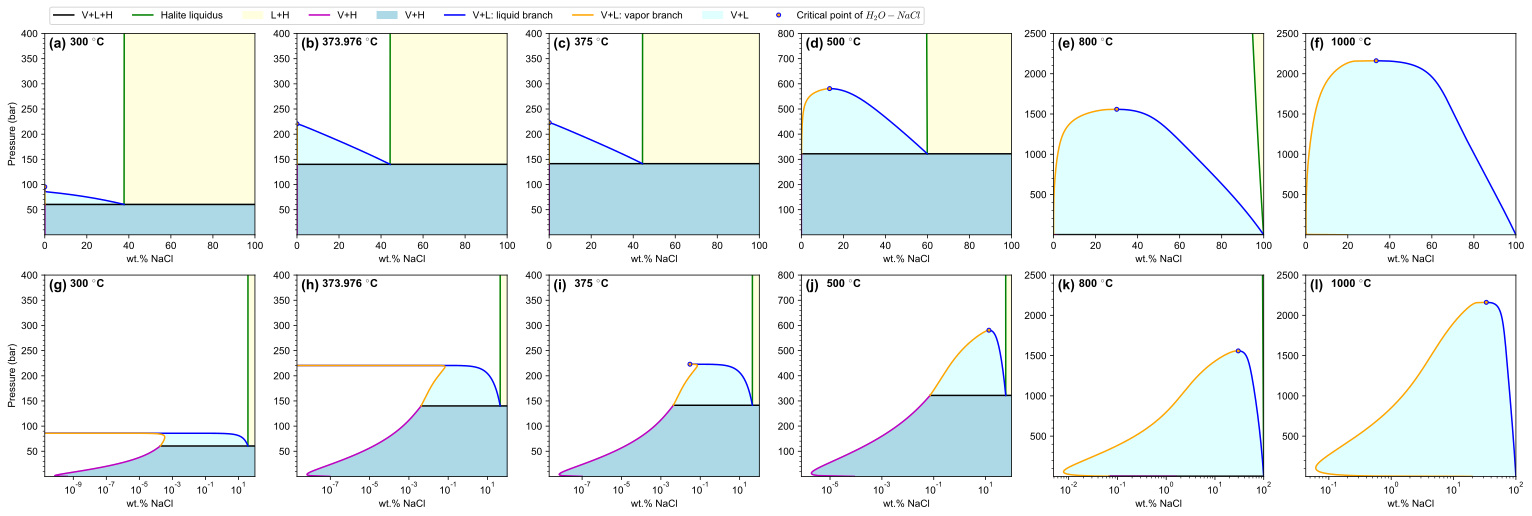
\includegraphics[width=\textwidth]{H2ONaCl_isothermal_PX.pdf}
			\caption{Isothermal pressure-composition sections.}
		\end{figure}
	
	\end{frame}

    % background and motivation
	\section{Background and motivation}
	\begin{frame}{Concept model}
	    
	\end{frame}
	
	\section{Development and issues}
	\begin{frame}{Main framework}
	    
	\end{frame}
	
	\begin{frame}{}
    \centering {\huge \color{GoogleRed} \textbf{\calligra{Thank You for Your Attention}}}
    \end{frame}
	% references
    \bibliography{ref/refs.bib}
\end{document} 